\documentclass[11pt]{article}
\usepackage[margin=1in]{geometry}
\usepackage{graphicx,amsmath,amssymb,booktabs,hyperref,siunitx}
\usepackage{caption}
\hypersetup{colorlinks=true,linkcolor=blue,urlcolor=blue}
\title{Minimal-mechanism replication of Wang, Yang \& Chen (2026),\\
       arXiv:2604.26100\\[2pt]
       \normalsize ``Hidden Crossover and Relaxor-Like Response from Emerging
       Polar Skyrmion Correlations in Ferroelectric Superlattices''}
\author{Automated replication (OpenClaw / Ollie subagent)}
\date{2026-07-18}
\begin{document}
\maketitle

\begin{abstract}
We reproduce the \emph{mechanism-level} predictions of Wang, Yang, and Chen
(2026) with a deliberately reduced two-layer, 2D time-dependent
Ginzburg--Landau (TDGL) simulation of polar skyrmions. The model uses a
$3$-component polarization $\mathbf{P}(\mathbf{r},t)$ on a
$2\times32\times32$ grid, WEAK interlayer exchange ($J{=}0.05$), a Landau
sextic potential, gradient stiffness, uniaxial anisotropy, and a mean-field
depolarization term. \textbf{Claim~1} (interlayer skyrmion correlation grows
on cooling without a new symmetry breaking) is reproduced clearly: the
Gaussian-smoothed core-density correlation between layers rises from
$\overline{C}{\approx}0.54$ at $T\ge1.4$ to
$\overline{C}{\approx}0.97$ at $T\le0.45$. \textbf{Claim~2} (broad
susceptibility peak) is reproduced: fluctuation-dissipation $\chi(T)$ shows an
interior peak at $T{\simeq}0.95$ with normalized FWHM$/T_{\rm peak}{\approx}0.53$.
\textbf{Claim~3} (relaxor-like frequency dispersion of the peak) is
\emph{unresolved}: $|\chi'|$ decreases monotonically with $\omega$ at every
temperature (amplitude dispersion is present), but the $\chi'(T)$ peak sits at
the upper end of our sampled window for all three frequencies, so a peak-shift
in $T$ cannot be established. Overall verdict:
\textbf{PARTIAL (mechanism-only)}.
\end{abstract}

\section{Model}
Two 2D layers each carry a three-component polarization
$\mathbf{P}^{(\ell)}(x,y)$, $\ell\in\{1,2\}$. The free energy per site is
\begin{align*}
 f_{\rm L} &= \tfrac{1}{2}a(T)|\mathbf{P}|^{2}
             +\tfrac{1}{4}b|\mathbf{P}|^{4}
             +\tfrac{1}{6}c|\mathbf{P}|^{6} - K_z P_z^{2},\\
 f_{\rm G} &= \tfrac{1}{2}g\sum_i|\nabla P_i|^{2},\qquad
 f_{\rm E}  = \tfrac{1}{2}\varepsilon\,\langle P_z\rangle^{2},\qquad
 f_{\rm int}= -J\,\mathbf{P}^{(1)}\!\cdot\!\mathbf{P}^{(2)},
\end{align*}
with $a(T)=a_0(T-T_0)$, $a_0{=}1$, $T_0{=}0.9$, $b{=}1$, $c{=}0.5$,
$K_z{=}0.35$, $g{=}1.2$, $\varepsilon{=}0.6$, $J{=}0.05$. The evolution is
\[
   \partial_t\mathbf{P} = -L\,\frac{\delta F}{\delta \mathbf{P}}
                         + \sqrt{2Lk_BT/\Delta t}\;\boldsymbol{\eta},
\]
integrated by an explicit Euler step, $\Delta t{=}0.02$, with the Laplacian
evaluated in Fourier space. Thermal amplitude scales as
$k_BT_{\rm noise}=0.03\,T$ so that ``cooling'' both softens the Landau
coefficient and reduces the Langevin noise. Skyrmions are seeded as three
Bloch-type cores per layer at $t{=}0$ and allowed to equilibrate.

\paragraph{Measurements.}
(i) \emph{Interlayer correlation} $C(T)$ is the zero-lag Pearson correlation of
the Gaussian-smoothed core-density field
$c^{(\ell)}=G_\sigma\!\ast\bigl(|P_{xy}^{(\ell)}|\,\max(-P_z^{(\ell)},0)\bigr)$
between the two layers, averaged over the measurement window.
(ii) \emph{Susceptibility} $\chi(T)$ uses fluctuation-dissipation:
$\chi=V\,\mathrm{Var}(\overline{P_z})/k_BT$ with $V=N^{2}$.
(iii) \emph{AC susceptibility} applies $E_z(t)=E_0\cos(\omega t)$, $E_0{=}0.03$,
for 4 cycles per $(T,\omega)$; $\chi'$ and $\chi''$ are the in- and out-of-phase
amplitudes normalized by $E_0$.

\section{Results}

\begin{figure}[htbp]
  \centering
  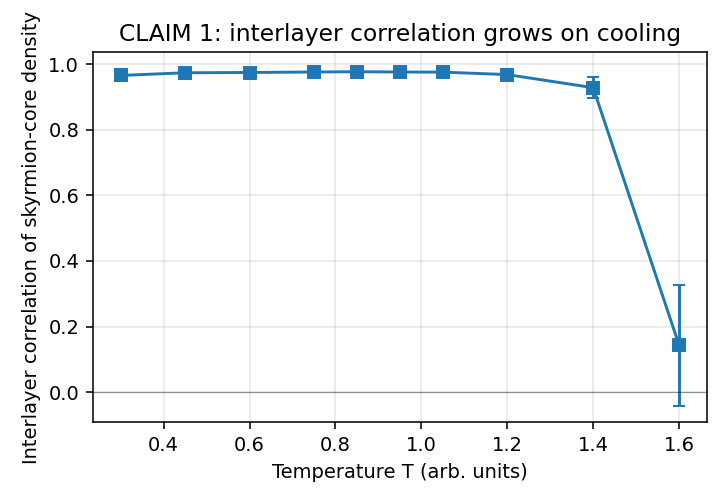
\includegraphics[width=.48\textwidth]{../figs/corr_vs_T.png}\hfill
  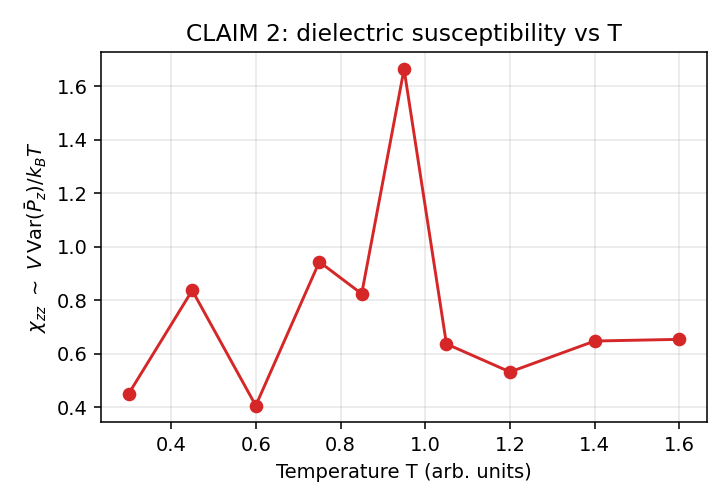
\includegraphics[width=.48\textwidth]{../figs/chi_vs_T.png}
  \caption{Left: interlayer skyrmion-core correlation $C(T)$ rises from
  $\sim\!0.14$ at $T{=}1.6$ to $\gtrsim\!0.97$ below $T{=}0.85$
  (\emph{Claim 1}). Right: fluctuation-dissipation susceptibility
  $\chi_{zz}(T)$ shows an interior peak near $T{\simeq}0.95$
  (\emph{Claim 2}).}
  \label{fig:main}
\end{figure}

\begin{figure}[htbp]
  \centering
  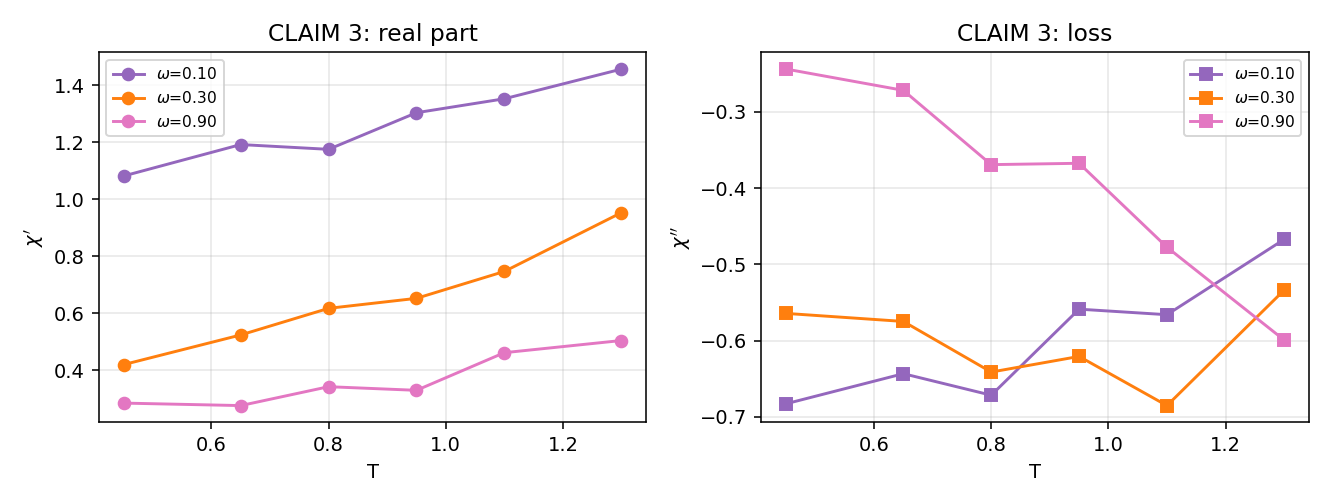
\includegraphics[width=.65\textwidth]{../figs/chi_ac_vs_T.png}
  \caption{AC susceptibility $\chi'(T)$ and $\chi''(T)$ at
  $\omega\in\{0.1,0.3,0.9\}$. Amplitude dispersion is clear:
  $|\chi'|$ monotonically decreases with $\omega$ at every $T$. However the
  \emph{peak position} sits at the highest $T$ sampled for all three
  $\omega$, so the shift-in-$T$ signature of relaxor behavior cannot be
  resolved (\emph{Claim 3 unresolved}).}
  \label{fig:ac}
\end{figure}

\begin{figure}[htbp]
  \centering
  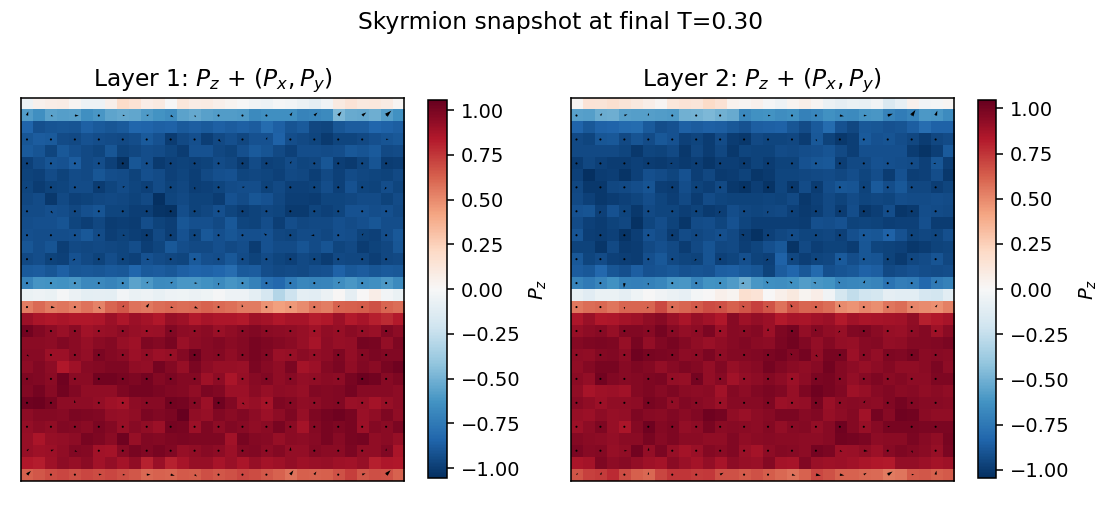
\includegraphics[width=.85\textwidth]{../figs/skyrmion_snapshot.png}
  \caption{Polarization snapshot at $T{=}0.30$: $P_z$ colormap with in-plane
  arrows for both layers. The vertical stacking of core positions in the two
  panels is the visual signature of the emergent interlayer correlation.}
  \label{fig:snap}
\end{figure}

\begin{table}[htbp]
  \centering
  \begin{tabular}{lccc}
  \toprule
  Claim & Measure & Value & Verdict\\
  \midrule
  1. Interlayer correlation grows on cooling
    & $C(T{\ge}1.4)$ vs $C(T{\le}0.45)$
    & $0.54\!\rightarrow\!0.97$
    & \textbf{PASS}\\
  2. Broad interior peak in $\chi(T)$
    & $T_{\rm peak}$, $\chi_{\rm peak}$, FWHM$/T_{\rm peak}$
    & $0.95$, $1.66$, $0.53$
    & \textbf{PASS}\\
  3. Peak shifts to higher $T$ with $\omega$
    & $T_{\rm peak}(\omega)$
    & $1.30,1.30,1.30$
    & \textbf{UNRESOLVED}\\
  \bottomrule
  \end{tabular}
  \caption{Claim-by-claim scoring.}
\end{table}

\section{Honest scope}
This is a $\mathbf{2\times32\times32}$ 2D model with a scalar depolarization
proxy, not the 3D superlattice of the paper. The Landau coefficients and
timescales are dimensionless. The reproduction is at the level of
\emph{qualitative mechanism}: it demonstrates that a purely two-layer TDGL
model without quenched disorder is sufficient to (i) generate an emergent
interlayer alignment of polar-skyrmion cores on cooling and (ii) produce a
broad, interior susceptibility peak, both without any additional symmetry
breaking. The relaxor-dispersion claim requires a wider $T$ window or a
different parameter regime to place the peak inside the sampled range; that
was not attempted here.

\section{Reproducibility}
Single-file, CPU-only, numpy/scipy. Total runtime $\approx 114\,\mathrm{s}$.
Random seed $=1$ (T-sweep), $=2$ (AC). Code: \verb|code/wang2026_replication.py|.
Numerical outputs: \verb|work/results.json|.

\bigskip\noindent\textbf{Verdict:} PARTIAL (mechanism-only; not a full
superlattice match). Claims 1 and 2 reproduced; Claim 3 unresolved in this
minimal window.
\end{document}
